\documentclass[12pt,a4paper]{article}

\usepackage[a4paper,margin=0.7in]{geometry}
\usepackage[T1]{fontenc}
\usepackage[utf8]{inputenc}
\usepackage{xcolor}
\usepackage{tikz}
\usepackage{float}
\usepackage{caption}
\usepackage{pdflscape}
\usetikzlibrary{arrows.meta, positioning, shadows, fit, backgrounds, calc}

\DeclareRobustCommand{\code}[1]{\texttt{\detokenize{#1}}}
\captionsetup{font=small,labelfont=bf}
\setlength{\emergencystretch}{4em}
\newif\ifexportdiagrams
\ifdefined\EXPORTDIAGRAMS
  \exportdiagramstrue
\else
  \exportdiagramsfalse
\fi

% Matches the colour language already used by the thesis runtime section:
% dialogue = blue, grounding/evidence = orange, planning = green,
% execution = purple, skills = neutral grey.
\colorlet{layerDialogue}{blue!7}
\colorlet{layerGrounding}{orange!10}
\colorlet{layerPlanner}{green!8}
\colorlet{layerExec}{purple!7}
\colorlet{layerSkill}{gray!5}
\colorlet{layerFuture}{red!6}
\colorlet{lineMain}{black!70}
\colorlet{lineEvidence}{orange!75!black}
\colorlet{lineFeedback}{brown!75!black}
\colorlet{lineAdapter}{purple!70!black}
\colorlet{lineFuture}{black!45}

\tikzset{
  outerBox/.style={
    draw=black!45,
    dashed,
    very thick,
    rounded corners=6pt,
    fill=gray!2,
    inner sep=6pt
  },
  subsystem/.style={
    draw=black!35,
    thick,
    rounded corners=5pt,
    fill=white,
    inner sep=5pt
  },
  nodebox/.style={
    draw=lineMain,
    thick,
    rounded corners=2pt,
    align=center,
    minimum height=10mm,
    inner xsep=3pt,
    inner ysep=4pt,
    font=\scriptsize,
    fill=white,
    drop shadow={shadow xshift=.45pt, shadow yshift=-.45pt, opacity=.12}
  },
  actor/.style={nodebox, fill=white, text width=22mm},
  dialogueNode/.style={nodebox, fill=layerDialogue, text width=22mm},
  groundingNode/.style={nodebox, fill=layerGrounding, text width=23mm},
  plannerNode/.style={nodebox, fill=layerPlanner, text width=24mm},
  execNode/.style={nodebox, fill=layerExec, text width=25mm},
  skillNode/.style={nodebox, fill=layerSkill, text width=20mm},
  futureNode/.style={nodebox, dashed, fill=layerFuture, text width=28mm},
  bus/.style={
    draw=black!45,
    thick,
    rounded corners=3pt,
    fill=gray!7,
    align=center,
    font=\scriptsize,
    inner ysep=3pt,
    inner xsep=5pt
  },
  control/.style={-{Latex[length=2.4mm,width=1.5mm]}, very thick, draw=lineMain},
  evidence/.style={-{Latex[length=2.2mm,width=1.4mm]}, thick, dashed, draw=lineEvidence},
  feedback/.style={-{Latex[length=2.2mm,width=1.4mm]}, thick, dashed, draw=lineFeedback},
  adapter/.style={-{Latex[length=2.2mm,width=1.4mm]}, thick, draw=lineAdapter},
  future/.style={-{Latex[length=2.0mm,width=1.2mm]}, thick, dashed, draw=lineFuture}
}

\begin{document}
\ifexportdiagrams\pagestyle{empty}\fi

% Add \usepackage{pdflscape} to main.tex, then paste the landscape figure.

\begin{landscape}
\begin{figure}[p]
\centering
\resizebox{0.98\linewidth}{!}{%
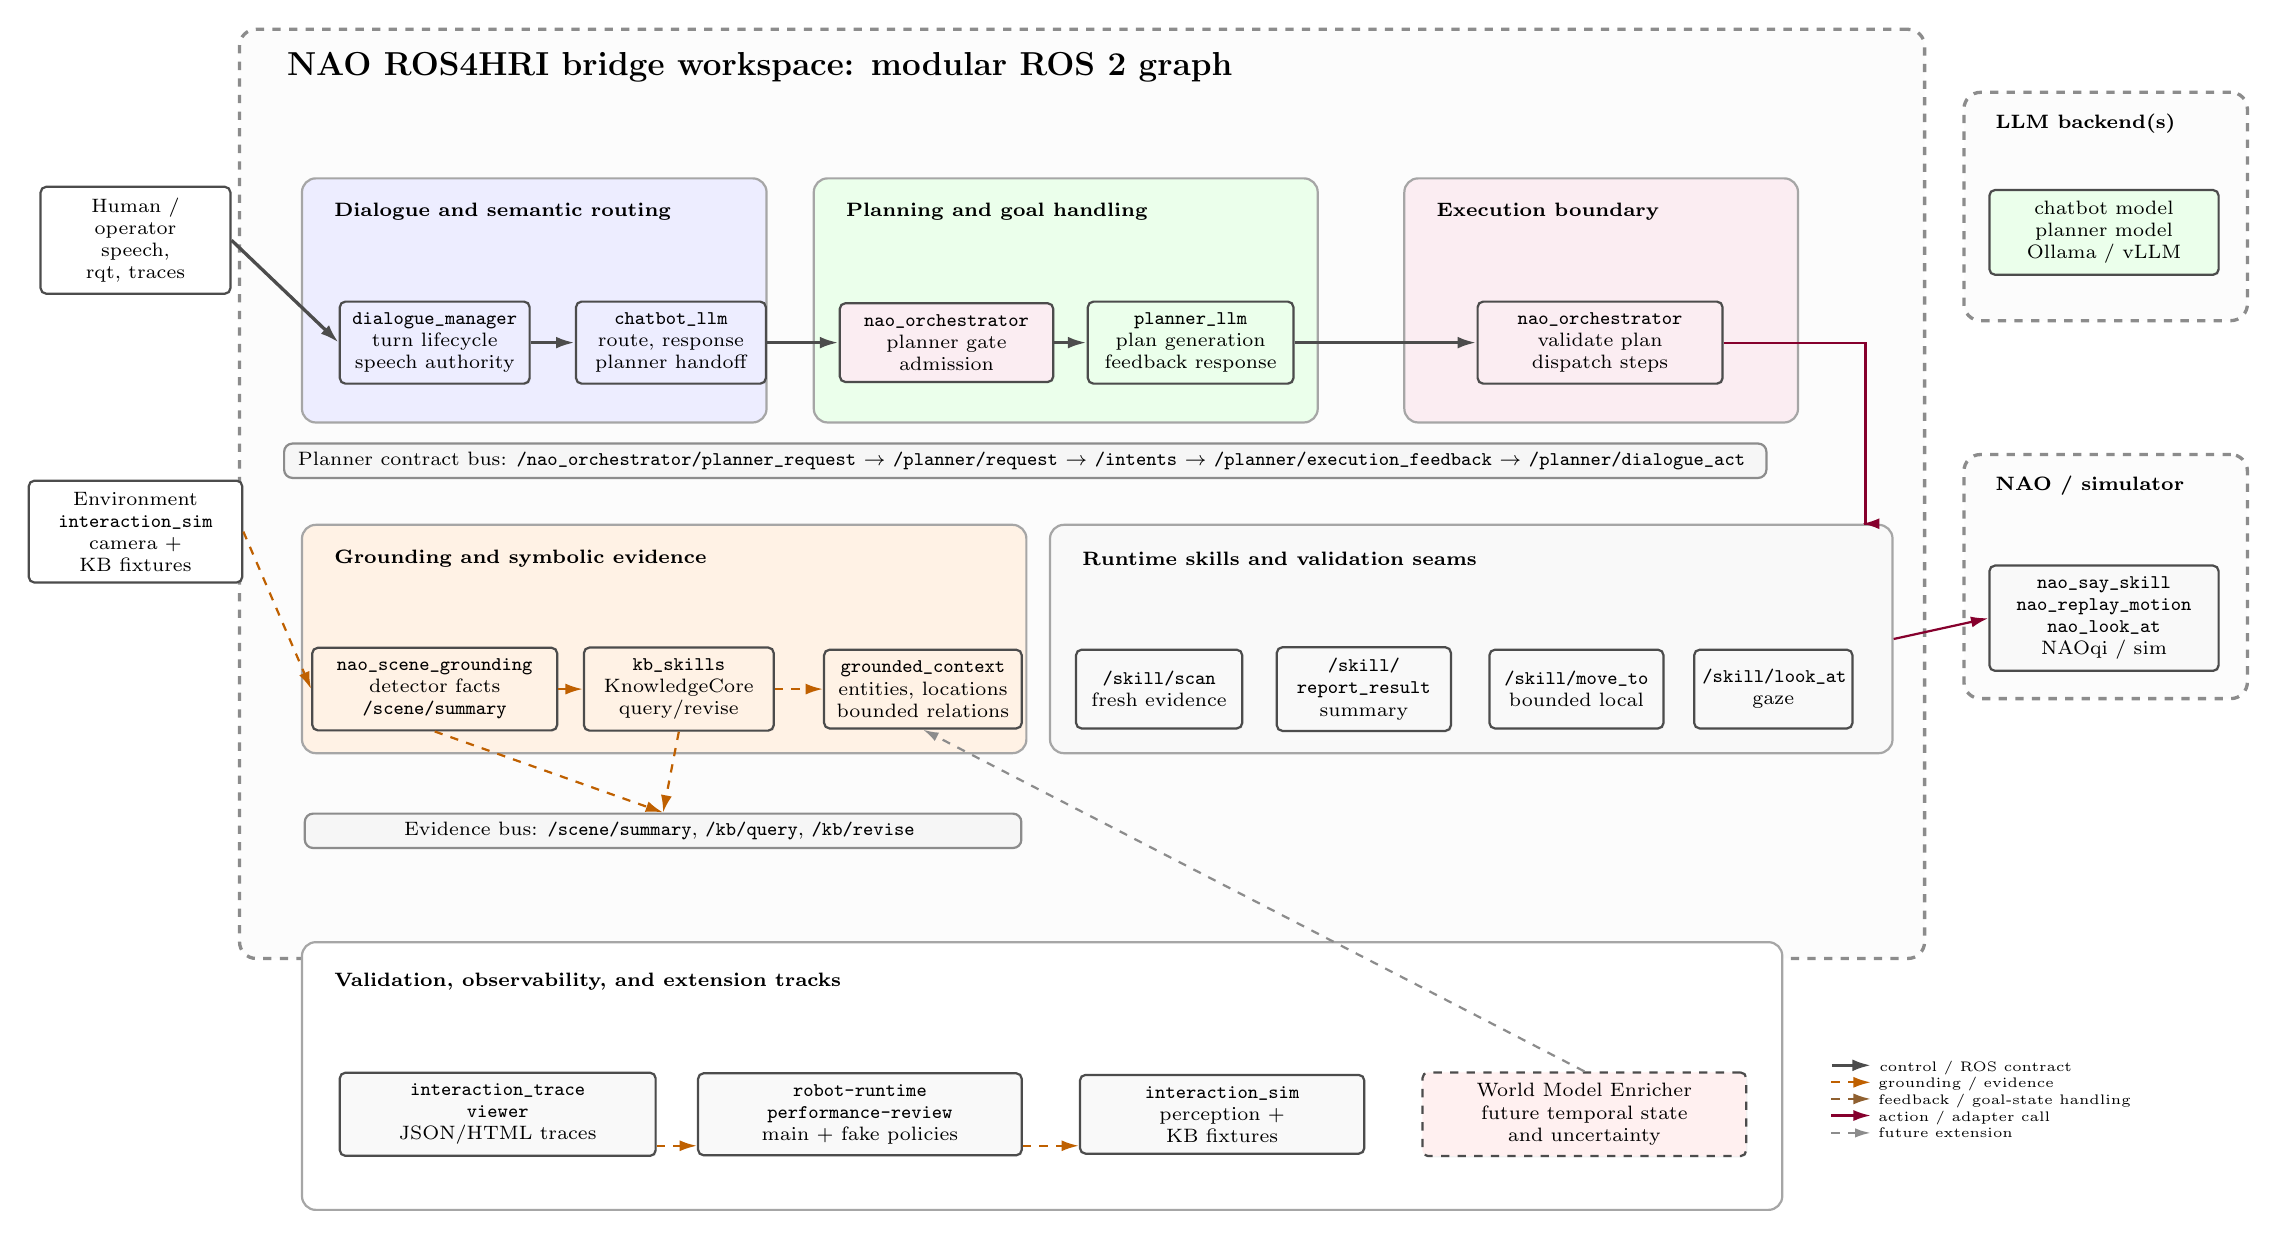
\begin{tikzpicture}[x=1mm,y=1mm]
  % Outer workspace boundary.
  \node[outerBox, minimum width=214mm, minimum height=118mm, anchor=north west] (workspace) at (23,124) {};
  \node[font=\large\bfseries, anchor=west] at (28,119) {NAO ROS4HRI bridge workspace: modular ROS 2 graph};

  % External context boxes.
  \node[actor] (human) at (10,97) {Human / operator\\speech, rqt, traces};
  \node[actor, text width=25mm] (environment) at (10,60) {Environment\\\code{interaction_sim}\\camera + KB fixtures};
  \node[outerBox, minimum width=36mm, minimum height=29mm, anchor=north west] (llmBox) at (242,116) {};
  \node[font=\scriptsize\bfseries, anchor=west] at (245,111.8) {LLM backend(s)};
  \node[nodebox, fill=layerPlanner, text width=27mm] (llm) at (260,98) {chatbot model\\planner model\\Ollama / vLLM};
  \node[outerBox, minimum width=36mm, minimum height=31mm, anchor=north west] (robotBox) at (242,70) {};
  \node[font=\scriptsize\bfseries, anchor=west] at (245,65.8) {NAO / simulator};
  \node[nodebox, fill=layerSkill, text width=27mm] (robot) at (260,49) {\code{nao_say_skill}\\\code{nao_replay_motion}\\\code{nao_look_at}\\NAOqi / sim};

  % Control-plane subsystems.
  \node[subsystem, fill=layerDialogue, minimum width=59mm, minimum height=31mm, anchor=north west] (dialogueArea) at (31,105) {};
  \node[font=\scriptsize\bfseries, anchor=west] at (34,100.6) {Dialogue and semantic routing};
  \node[dialogueNode] (dm) at (48,84) {\code{dialogue_manager}\\turn lifecycle\\speech authority};
  \node[dialogueNode] (chatbot) at (78,84) {\code{chatbot_llm}\\route, response\\planner handoff};

  \node[subsystem, fill=layerPlanner, minimum width=64mm, minimum height=31mm, anchor=north west] (planningArea) at (96,105) {};
  \node[font=\scriptsize\bfseries, anchor=west] at (99,100.6) {Planning and goal handling};
  \node[execNode] (gate) at (113,84) {\code{nao_orchestrator}\\planner gate\\admission};
  \node[plannerNode] (planner) at (144,84) {\code{planner_llm}\\plan generation\\feedback response};

  \node[subsystem, fill=layerExec, minimum width=50mm, minimum height=31mm, anchor=north west] (executionArea) at (171,105) {};
  \node[font=\scriptsize\bfseries, anchor=west] at (174,100.6) {Execution boundary};
  \node[execNode, text width=29mm] (orchestrator) at (196,84) {\code{nao_orchestrator}\\validate plan\\dispatch steps};

  % Contract bus separated from the nodes.
  \node[bus, minimum width=176mm] (plannerBus) at (123,69) {
    Planner contract bus:
    \code{/nao_orchestrator/planner_request} \(\rightarrow\)
    \code{/planner/request} \(\rightarrow\) \code{/intents} \(\rightarrow\)
    \code{/planner/execution_feedback} \(\rightarrow\) \code{/planner/dialogue_act}
  };

  % Evidence row.
  \node[subsystem, fill=layerGrounding, minimum width=92mm, minimum height=29mm, anchor=north west] (groundingArea) at (31,61) {};
  \node[font=\scriptsize\bfseries, anchor=west] at (34,56.6) {Grounding and symbolic evidence};
  \node[groundingNode, text width=29mm] (scene) at (48,40) {\code{nao_scene_grounding}\\detector facts\\\code{/scene/summary}};
  \node[groundingNode, text width=22mm] (kb) at (79,40) {\code{kb_skills}\\KnowledgeCore\\query/revise};
  \node[groundingNode] (context) at (110,40) {\code{grounded_context}\\entities, locations\\bounded relations};

  \node[bus, minimum width=91mm] (evidenceBus) at (77,22) {
    Evidence bus: \code{/scene/summary}, \code{/kb/query}, \code{/kb/revise}
  };

  % Skills row.
  \node[subsystem, fill=layerSkill, minimum width=107mm, minimum height=29mm, anchor=north west] (skillsArea) at (126,61) {};
  \node[font=\scriptsize\bfseries, anchor=west] at (129,56.6) {Runtime skills and validation seams};
  \node[skillNode, text width=19mm] (scan) at (140,40) {\code{/skill/scan}\\fresh evidence};
  \node[skillNode, text width=20mm] (report) at (166,40) {\code{/skill/}\\\code{report_result}\\summary};
  \node[skillNode, text width=20mm] (move) at (193,40) {\code{/skill/move_to}\\bounded local};
  \node[skillNode, text width=18mm] (look) at (218,40) {\code{/skill/look_at}\\gaze};

  % Validation and future row.
  \node[subsystem, fill=white, minimum width=188mm, minimum height=34mm, anchor=north west] (validationArea) at (31,8) {};
  \node[font=\scriptsize\bfseries, anchor=west] at (34,2.8) {Validation, observability, and extension tracks};
  \node[skillNode, text width=38mm] (trace) at (56,-14) {\code{interaction_trace}\\\code{viewer}\\JSON/HTML traces};
  \node[skillNode, text width=39mm] (review) at (102,-14) {\code{robot-runtime}\\\code{performance-review}\\main + fake policies};
  \node[skillNode, text width=34mm] (simprofile) at (148,-14) {\code{interaction_sim}\\perception +\\KB fixtures};
  \node[futureNode, text width=39mm] (wme) at (194,-14) {World Model Enricher\\future temporal state\\and uncertainty};

  % Primary sequential control path.
  \draw[control] (human.east) -- (dm.west);
  \draw[control] (dm.east) -- (chatbot.west);
  \draw[control] (chatbot.east) -- (gate.west);
  \draw[control] (gate.east) -- (planner.west);
  \draw[control] (planner.east) -- (orchestrator.west);

  % Grounding and compact context paths.
  \draw[evidence] (environment.east) -- (scene.west);
  \draw[evidence] (scene.east) -- (kb.west);
  \draw[evidence] (kb.east) -- (context.west);
  \draw[evidence] (scene.south) -- (evidenceBus.north);
  \draw[evidence] (kb.south) -- (evidenceBus.north);

  % Skill execution and feedback.
  \draw[adapter] (orchestrator.east) -- ++(18,0) |- ([xshift=-4mm]skillsArea.north east);
  \draw[adapter] (skillsArea.east) -- (robot.west);

  % Observability and extension paths.
  \draw[evidence] ([yshift=-4mm]trace.east) -- ([yshift=-4mm]review.west);
  \draw[evidence] ([yshift=-4mm]review.east) -- ([yshift=-4mm]simprofile.west);
  \draw[future] (wme.north) -- (context.south);

  % The backend is a deployment callout: chatbot_llm and planner_llm call it,
  % but the arrows are intentionally omitted here to keep the architecture plate
  % readable beside the more detailed runtime sequence diagram.

  % Legend.
  \node[align=left, font=\tiny, anchor=west] at (224,-12) {
    \tikz{\draw[control] (0,0)--(5mm,0);} control / ROS contract\\
    \tikz{\draw[evidence] (0,0)--(5mm,0);} grounding / evidence\\
    \tikz{\draw[feedback] (0,0)--(5mm,0);} feedback / goal-state handling\\
    \tikz{\draw[adapter] (0,0)--(5mm,0);} action / adapter call\\
    \tikz{\draw[future] (0,0)--(5mm,0);} future extension
  };
\end{tikzpicture}%
}
\ifexportdiagrams\else
  \caption{High-level full-stack architecture of the implemented NAO ROS4HRI bridge. The diagram complements the runtime sequence view by emphasizing subsystem ownership, deployment boundaries, ROS contract buses, validation seams, and the future World Model Enricher. The colour coding follows the thesis runtime section: dialogue components are blue, grounding and evidence are orange, planning is green, execution is purple, and skill/adaptor nodes are neutral grey.}
  \label{fig:full-stack-architecture-plate}
\fi
\end{figure}
\end{landscape}

\end{document}
